
\chap{Results}

The main result of this work is the implemented "Python Analyzer System" itself. It actually provides an automatic way to make an initial analysis and display the results of any input dataset.

Further more has been provided an initial Python implementation of:
\begin{itemize}
\item Future Prediction System
\item Country Map Displaying System
\end{itemize}
\newpage

\begin{figure}[H]
	\centering
    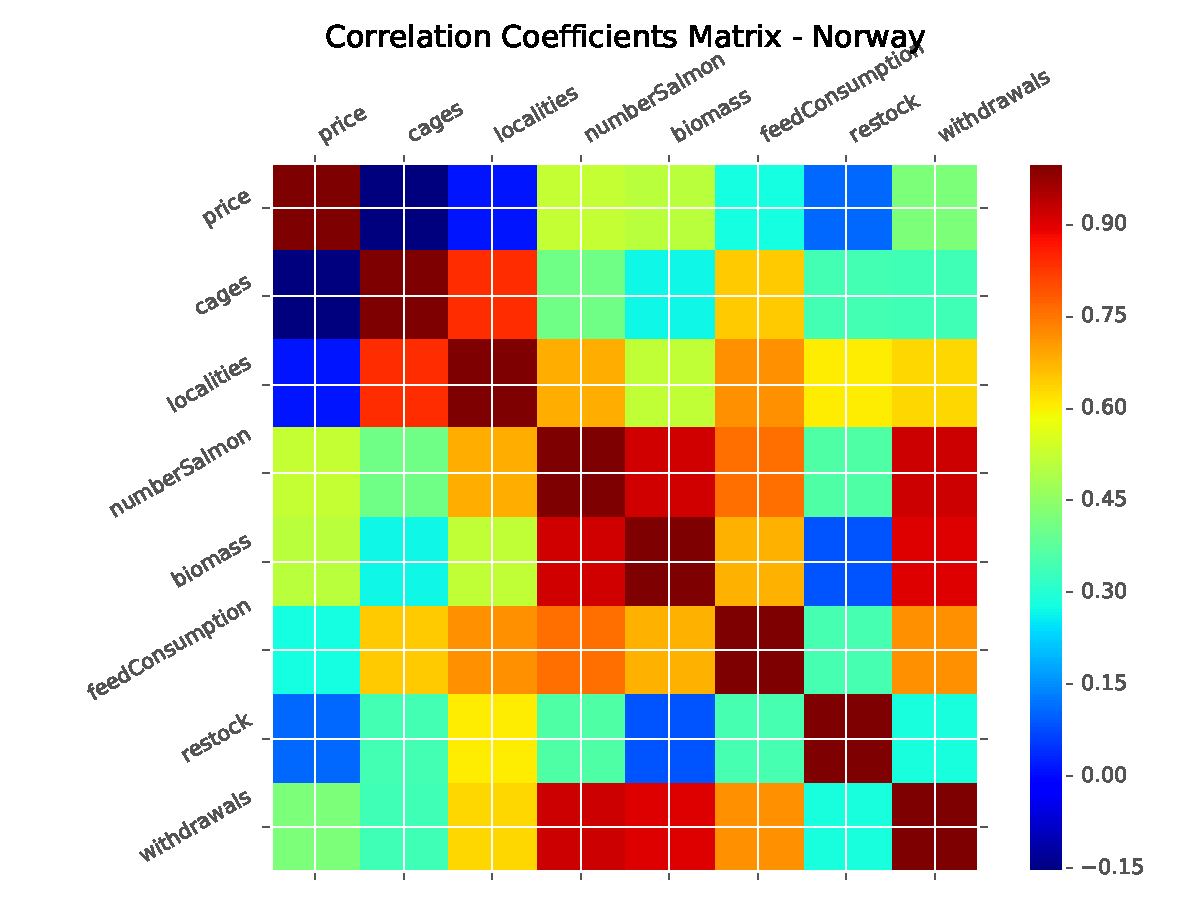
\includegraphics[width=1\textwidth]{Files/Total_Dataset_Matrix.pdf}
    \caption{Correlation matrix between different inputs with data from 2005 to 2016.}
\end{figure}

\begin{table}[ht] 
\makebox[\textwidth][c] {
\resizebox{1.2\textwidth}{!}{\begin{tabular}{ | l | l | l | l | l | l | l | l | l |}
        \hline
INPUTS	& Price 		& Cages 			& Localities		& numberSalmon 		& biomass 		& feedConsumption 		& restock 		& withdrawals 				\\ \hline
Price			& 1			& -0.16		& 0.02 		& 0.52		& 0.51		& 0.28		& 0.11 		& 0.43		\\ \hline
Cages			& -0.16		& 1			& 0.84		& 0.41		& 0.27		& 0.64		& 0.34		& 0.34		\\ \hline
Localities		& 0.02		& 0.84		& 1			& 0.68		& 0.52		& 0.72		& 0.6		& 0.63		\\ \hline
numberSalmon	& 0.52		& 0.41		& 0.68		& 1 		& 0.92		& 0.76		& 0.36		& 0.92		\\ \hline
biomass			& 0.51		& 0.27		& 0.52		& 0.92		& 1			& 0.68		& 0.09		& 0.91		\\ \hline
feedConsumption	& 0.28		& 0.64		& 0.72		& 0.76		& 0.68		& 1			& 0.35		& 0.72		\\ \hline
restock			& 0.11		& 0.34		& 0.6		& 0.36		& 0.09		& 0.35		& 1 		& 0.28		\\ \hline
withdrawals		& 0.43		& 0.34		& 0.63		& 0.92		& 0.91		& 0.72		& 0.28		& 1			\\ \hline
    \end{tabular}}}
    \caption{Dataset inputs correlation coefficients value.}
    \label{table: trendline} 
\end{table}

\newpage

\begin{figure}[H]
	\centering
    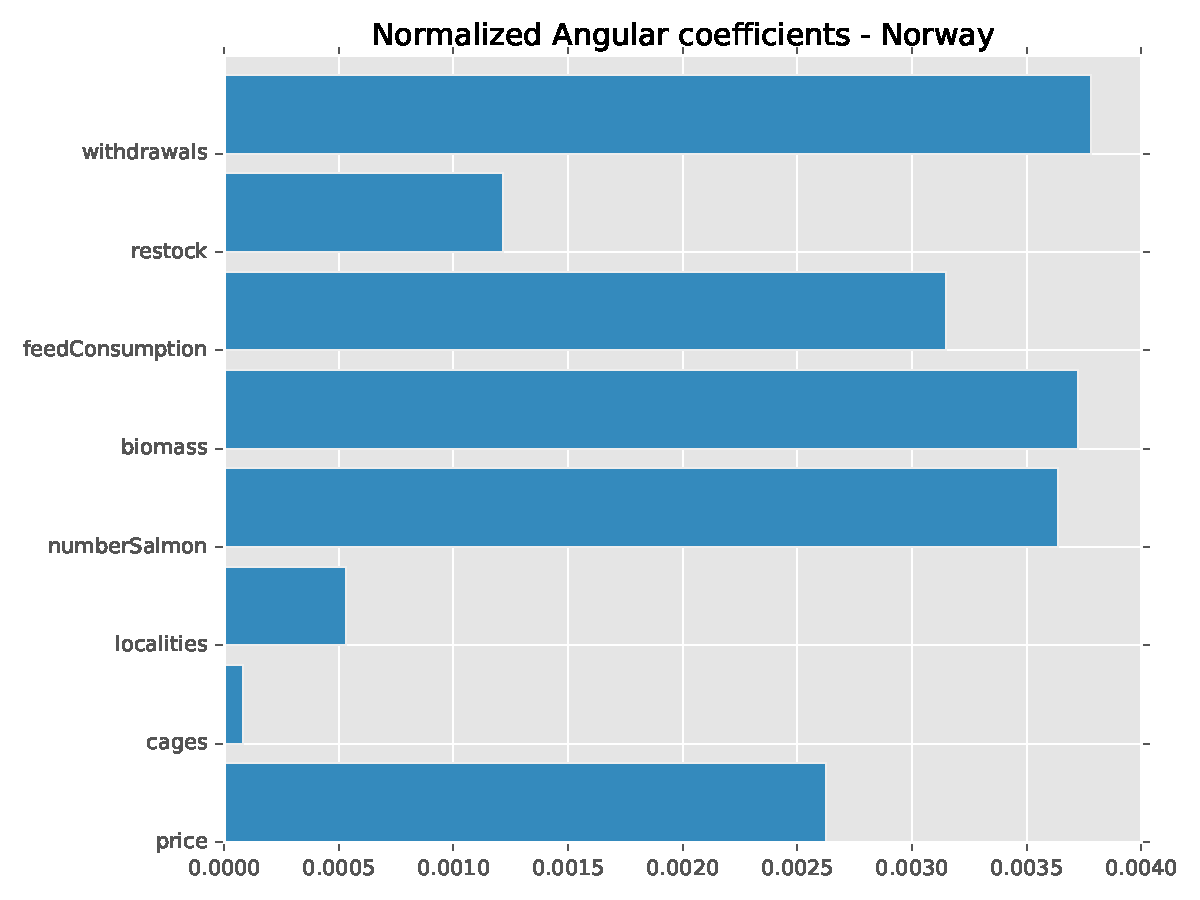
\includegraphics[width=1\textwidth]{Files/Norm_Ang_Coeffs.pdf}
    \caption{Normalized angular coefficients of each input's trendline.}
\end{figure}

\begin{table}[ht] 
	\centering
    \begin{tabular}{ | l | l | l | p{5cm} |}
        \hline
        Input 								& Equation 							& Coeff			\\ \hline
          	Salmon\_withdrawals 			& y=464.755139x+(46295.729945) 		& 464.755139 	\\ \hline
          	Salmon\_biomass\_end\_month 	& y=2832.712270x+(354138.727889) 	& 2832.71227 	\\ \hline
          	Salmon\_number\_end\_month 		& y=1543.298421x+(205325.455772)	& 1543.298421 	\\ \hline
          	Salmon\_consumption\_of\_feed 	& y=620.070855x+(58330.012273) 		& 620.070855	\\ \hline
           	Salmon\_price 			& y=0.178175x+(22.643654)			& 0.1781753878 		\\ \hline
          	Salmon\_restock 				& y=89.230600x+(13390.363406)		& 89.2306 		\\ \hline
 			Localities 						& y=0.343533x+(539.979023) 			& 0.343533		\\ \hline
  			Cages 							& y=0.342834x+(3665.904023) 		& 0.342834 		\\ \hline
    \end{tabular} 
    \caption{Dataset inputs trendline equation}
    \label{table: trendline} 
\end{table}
\begin{table}[ht] 
	\centering
    \begin{tabular}{ | l | l | l | p{5cm} |}
        \hline
        Input 							& Normalized equation 	& Norm Ang Coeffs	\\ \hline
          	Salmon\_withdrawals 		& y=0.003782x+(0.376694)& 0.003782			\\ \hline
          	Salmon\_biomass\_end\_month & y=0.003724x+(0.465599)& 0.003724			\\ \hline
          	Salmon\_number\_end\_month 	& y=0.003639x+(0.484184)& 0.003639			\\ \hline
          	Salmon\_consumption\_of\_feed & y=0.003147x+(0.296085)& 0.003147		\\ \hline
           	Salmon\_price 		& y=0.002625x+(0.333633)
& 0.002625			\\ \hline
          	Salmon\_restock 			& y=0.001217x+(0.182583)& 0.001217			\\ \hline
 			Localities 					& y=0.000531x+(0.834589)& 0.000531			\\ \hline
  			Cages 						& y=0.000082x+(0.877011)& 0.000082			\\ \hline
    \end{tabular} 
    \caption{Dataset inputs normalized trendline equation}
    \label{table: norm_trendline} 
\end{table}

\newpage

\begin{figure}[H]
    \makebox[\textwidth][c]{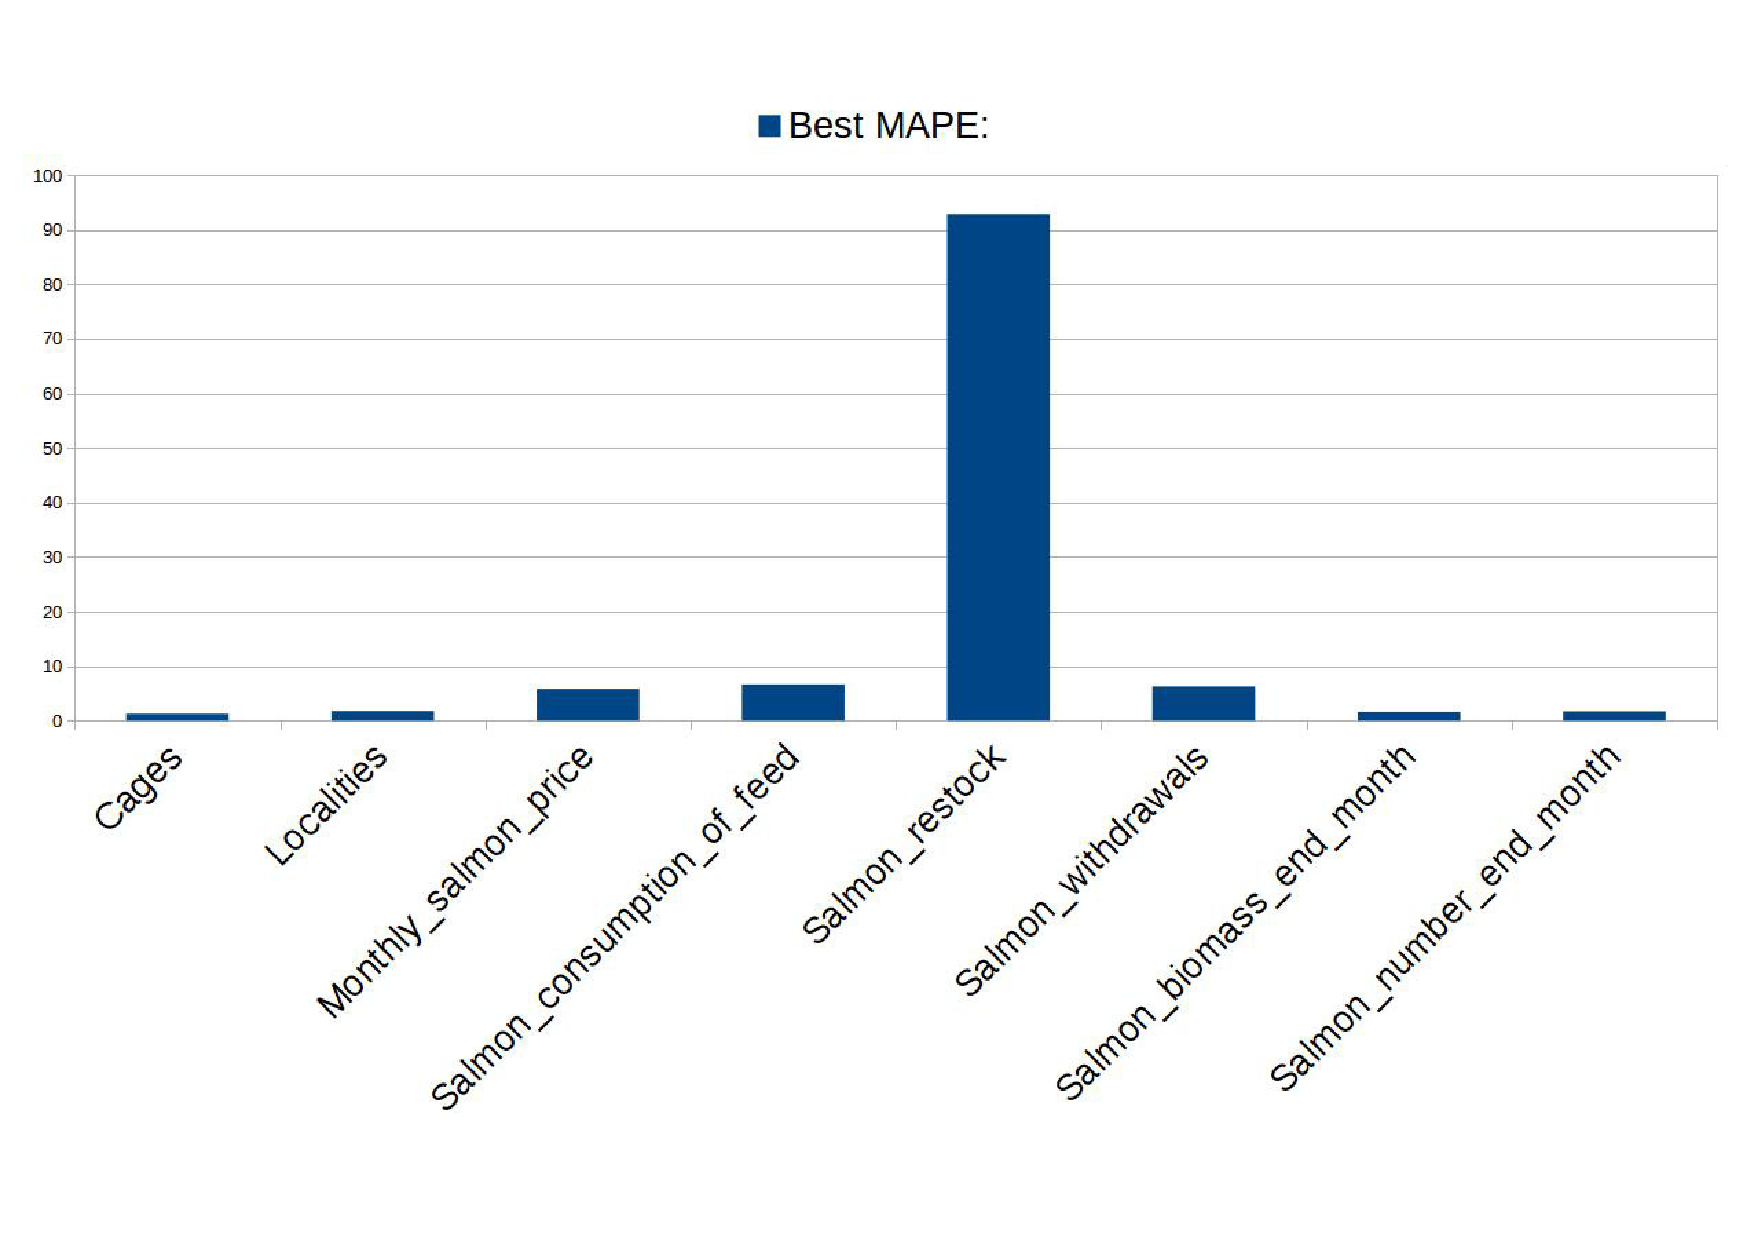
\includegraphics[width=1.2\textwidth]{Files/Best_MAPE.pdf}}
    \caption{Lower MAPE with best ARIMA Configuration for each tested input.}
\end{figure}

\begin{table}[ht] 
	\centering
    \begin{tabular}{ | l | l | l |}
            \hline
Input							&	ARIMA Conf	&	MAPE	\\ \hline
Cages							&	(10,2,1)	&	1.251\%	\\ \hline
Localities						&	(10,0,1)	&	1.779\%	\\ \hline
Salmon\_price 					&	(0,1,1)		&	6.686\%	\\ \hline
Salmon\_consumption\_of\_feed	&	(6,1,0)		&	6.659\%	\\ \hline
Salmon\_restock 				&	(10,0,1)	&	96.006\%	\\ \hline
Salmon\_withdrawals 			&	(10,0,1)	&	6.277\%	\\ \hline
Salmon\_biomass\_end\_month		&	(8,1,0)		&	1.601\%	\\ \hline
Salmon\_number\_end\_month 		&	(10,2,0)	&	1.723\%	\\ \hline
    \end{tabular}  
    \caption{Dataset inputs normalized trendline equation}
    \label{table: Best ARIMA configurations with relative MAPE result in the Evaluation Test} 
\end{table}

\newpage

\makebox[\textwidth][c]{
\resizebox{1.3\textwidth}{!}{
\begin{tabular}{|c|c|c|c|c|c|c|c|c|c|c|c|c|c|}
\hline
\multirow{3}{*}{Months} & \multicolumn{3}{c|}{Cages} & \multicolumn{3}{c|}{Localities} & \multicolumn{3}{c|}{Salmon Biomass} & \multicolumn{3}{c|}{Salmon Number}\\
\cline{2-13}
 & Real & Pred & Error & Real & Pred & Error & Real & Pred & Error & Real & Pred & Error \\
\hline
 January 2017 & 3436 & 3444.87 & 0.26\% & 539.000 & 543.41 & 0.82\% & 738902 & 732841.36 & 0.82\% & 369274 & 366826.189 & 0.66\%\\
\hline
 February 2017 & 3225 & 3251.915 & 0.83\% & 523.000 & 529.05 & 1.16\% & 712981 & 709931.42 & 0.43\% & 347824 & 352905.30 & 1.46\% \\
 \hline
 March 2017 & 3153 & 3164.190 & 0.67\% & 529.000 & 534.29 & 1.00\% & 667749 & 679405.11 & 1.75\% & 343636 & 349747.77 & 1.78\%\\
 \hline
 April 2017 & & 3317.814 & & & 549.14 & & & 657418.41 & & & 369616.83 &  \\
 \hline
 May 2017 & & 3492.701 & & & 550.64 & & & 646850.14 & & & 387244.43 &  \\
 \hline
 June 2017 & & 3507.062 & & & 545.66 & & & 653574.18 & & & 387630.48 & \\
 \hline
 July 2017 & & 3485.804 & & & 560.58 & & & 678469.77 & & & 384314.00 &  \\
 \hline
 August 2017 & & 3588.373 & & & 584.55 & & & 707646.99 & & & 394062.43 & \\
 \hline
 September 2017 & & 3751.633 & & & 596.32 & & & 734628.28 & & & 411164.01 & \\
 \hline
 October 2017 & & 3790.521 & & & 589.11 & & & 757679.66 & & & 411094.09 & \\
 \hline
 November 2017 & & 3710.033 & & & 576.75 & & & 770838.51 & & & 396102.24 & \\
 \hline
 December 2017 & & 3584.505 & & & 563.56 & & & 771279.10 & & & 380399.93 & \\
 \hline
% etc. ...
\end{tabular}  }}


\makebox[\textwidth][c]{
\resizebox{1.3\textwidth}{!}{
\begin{tabular}{|c|c|c|c|c|c|c|c|c|c|c|c|c|c|}
\hline
\multirow{3}{*}{Months} & \multicolumn{3}{c|}{Consumption of feed} & \multicolumn{3}{c|}{Salmon restock} & \multicolumn{3}{c|}{Salmon Withdrawals} & \multicolumn{3}{c|}{Salmon price}\\
\cline{2-13}
 & Real & Pred & Error & Real & Pred & Error & Real & Pred & Error & Real & Pred & Error \\
\hline
 January 2017 & 109341 & 98174.28 & 10.21\% & 4415 & 4734.43 & 7.23\% & 87609 & 90488.98 & 3.29\% & & &\\
\hline
 February 2017 & 88704 & 77998.20 & 12.07\% & 991 & 6904.51 & 596.72\% & 3.29\% & 101295.55 & 11.00\% & & &\\
 \hline
 March 2017 & 87033 & 74726.18 & 14.14\% & 13594 & 15427.63 & 13.49\% & 109498 & 101724.09 & 7.10\% & & &\\
 \hline
 April 2017 & & 88768.11 & & & 39781.36 & & & 95032.95 & & & &\\
 \hline
 May 2017 & & 113280.67 & & & 39438.14 & & & 92065.64 & & & &\\
 \hline
 June 2017 & & 140413.56 & & & 22562.89 & & & 88775.54 & & & &\\
 \hline
 July 2017 & & 164511.15 & & & 20449.85 & & & 92643.44 & & & &\\
 \hline
 August 2017 & & 179690.48 & & & 39487.67 & & & 104102.60 & & & &\\
 \hline
 September 2017 & & 181556.12 & & & 49991.91 & & & 110419.37 & & & &\\
 \hline
 October 2017 & & 169502.10 & & & 31449.69 & & & 107588.69 & & & &\\
 \hline
 November 2017 & & 147770.73 & & & 11698.23 & & & 102943.86 & & & &\\
 \hline
 December 2017 & & 123447.55 & & & 7957.45 & & & 99561.98 & & & &\\
 \hline
% etc. ...
\end{tabular}  }}


